% vim: tw=80 sw=2 ts=2 ff=unix spelllang=en spell
\documentclass{beamer}
\newcommand{\colA}[1]{\begin{columns}[t]\begin{column}{#1}}
\newcommand{\colB}[1]{\end{column}\begin{column}{#1}}
\newcommand{\colEnd}{\end{column}\end{columns}}

\usetheme{CambridgeUS}
\usecolortheme{dolphin}
%\setbeamercovered{transparent}
%\useoutertheme{infolines}

\usepackage{xltxtra}
\usepackage{fancyvrb}
%% \usepackage{ngerman}
\institute[]{Centrum für Informations- und Sprachverarbeitung (CIS)\\
            Ludwig-Maximilians-Universität München (LMU)\\
            \vspace{1cm}
            \href{https://creativecommons.org/licenses/by-nc-sa/4.0/}%
            {\includegraphics[width=0.2\textwidth]{../presentations/images/by-nc-sa.eps}}}

% keine Navigationspfeile
\setbeamertemplate{navigation symbols}{} % keine Navigations-Buttons

% Standardschrift verändern für Griechisch
%\setsansfont[Mapping=tex-text]{Junicode}
%\setmonofont[Mapping=tex-text]{DejaVu Sans Mono}
%\setsansfont[Mapping=tex-text]{Linux Libertine O}
%\setsansfont[Scale=MatchLowercase]{Linux Biolinum O}

% Fußzeile mit Titel und Seitenr.
\definecolor{mygray}{gray}{0.25}
%\setbeamertemplate{footline}[frame number]
\setbeamertemplate{footline}{\color{mygray}\hspace*{2mm}\insertauthor\hfill \insertshorttitle\hfill\insertdate\hspace*{10pt}\insertframenumber\ / \inserttotalframenumber\hspace*{2ex}}

% Schrift für URLs
\definecolor{myblue}{rgb}{0.2 0.0 0.8}

\usepackage{hyperref}
\renewcommand{\UrlFont}{\color{myblue}\footnotesize\sf}
\hypersetup{colorlinks,allcolors=.,urlcolor=blue}

% Bibliography
%\usepackage[backend=biber,style=authoryear,maxcitenames=2,maxbibnames=9]{biblatex}

% Schriftgröße Listings
\RequirePackage{fancyvrb}
\DefineVerbatimEnvironment{Highlighting}{Verbatim}%
  {commandchars=\\\{\},fontsize=\footnotesize}
\DefineVerbatimEnvironment{Verbatim}{Verbatim}%
  {fontsize=\footnotesize}
\newcommand{\pocoto}{\texttt{PoCoTo}}

\title{Datech 2017 -- \pocoto{} Workshop -- Profiler}
\author{Florian~Fink}

\begin{document}

\begin{frame}
	\titlepage
\end{frame}

\section{Profiling}
\subsection{Overview}
\begin{frame}
	\begin{itemize}
		\item OCR'ed historical Documents contain errors.
		\item Historical documents contain lots of spelling variation.
		\item If you want to find errors in OCR'ed documents, you need a fitting
			historical dictionary.
		\item If you only have a modern dictionary, you will get a lot of false
			positives (\emph{vnnd}, \emph{Thurm}, \dots).
	\end{itemize}
\end{frame}

\subsection{Language profiler}
\begin{frame}
	The language Profiler was created to help to find OCR-errors in OCR'ed
	historical documents and to generate correction candidates for suspected
	errors\footnote{Ulrich Reffle, 2011, \emph{Algorithmen und Methoden
	zur dokumentenspezifischen Analyse historischer und OCR-erfasster Texte}}.

	\begin{itemize}
		\item The profiler tries to distinguish real OCR-errors from historical
			spelling variants.
		\item The profiler uses various modern dictionaries.
		\item The profiler uses a (language-dependent) pattern list, that describes
			historical spelling variations.
		\item The profiler generates a document-dependent profile (the \emph{document
			profile}), that uses an expectation maximization algorithm to maximize the
			probabilities of the OCR and language patterns for a given document.
	\end{itemize}
\end{frame}

\subsection{Documentation}
\begin{frame}
	\begin{itemize}
		\item The profiler is documented in the
			\href{https://github.com/cisocrgroup/Resources/blob/master/manuals/profiler-manual.pdf}{profiler
			manual} (included in the workshop's data package).
		\item Its source is available on \href{https://github.com/cisocrgroup/Profiler}{github}.
		\item The profiling web service, that is used by \pocoto{} is also available
			on \href{https://github.com/cisocrgroup/ProfilerWebService}{github}.
		\item It needs Linux and different C++ development tools (cmake, make, g++,
			boost, xerces, \dots).
		\item The profiler contains various tools that compile different forms of
			dictionaries, perform lookup in different dictionaries and generate
			correction candidates for unknown words.
	\end{itemize}
\end{frame}

\subsection{Language backend}
\begin{frame}
	The profiler uses a so called \emph{language backend}, that contains the
	language dependent resources for the profiler. The language backend contains:
	\begin{itemize}
		\item A configuration file
		\item A collection of historical and modern compiled dictionaries.
		\item A historical pattern file
		\item A frequency list of a historical patterns from a ground
			truth\footnote{This is a bug, since this resource should be optional.}
	\end{itemize}
\end{frame}

\subsection{Resources}
\begin{frame}
	\begin{itemize}
		\item Dictionaries must be compiled from plain text files using the
			\texttt{compileFBDic}.
		\item The historical pattern file is a plain text file that lists various
			spelling variation patterns in the form: \texttt{modern:historical}.
		\item The frequency list must be compiled from a historical ground truth
			using the \texttt{trainFrequencyList} tool\footnote{You can use a small
			garbage file if you do not have a appropriate historical ground truth.}
	\end{itemize}
\end{frame}

\subsection{Pattern file}
\begin{frame}
	\begin{itemize}
		\item If you work with the profiler you will often recognize missing
			historical patterns.
		\item The simplest resource to update is the historical pattern list.
		\item It is a plain text file that can be edited.
		\item New patterns can be added easily to the pattern file.
	\end{itemize}
\end{frame}

\subsection{Example pattern file}
\begin{frame}[fragile]
	The pattern file is a plain text file with one pattern per line. Each pattern
	must be of the form \texttt{modern:hist}. You can use \texttt{\$} to mark end
	of words. Lines that start with \texttt{\#} are ignored:

\begin{verbatim}
# patterns.txt
# cases are ignored!
# turm was often spelled thurm
t:th
# teil was often spelled theyl
ei:ey
\end{verbatim}
\end{frame}

\subsection{Profiling a project}
\begin{frame}
	\begin{itemize}
		\item If you want to profile a document, make sure that you have
			configured a valid profiler web service url (see the
			\href{https://github.com/cisocrgroup/Resources/blob/master/manuals/profiler-manual.md}{profiler
			manual} for more information).
		\item You can always use the default profiler url of \pocoto{}.
		\item You can always profile your current project by clicking
			\texttt{profiler->order document profiler} in the menu area:
					\begin{itemize}
						\item If the url is valid and the profiler web service is running, you
							will see a window, which lets you choose which language profile
							to use.
						\item Select a language and click to \texttt{order document profile}.
						\item Do as \pocoto{} says and get your self some coffee.
					\end{itemize}
				\item After the profiling has stopped, you now will have access to the
					common error pattern tab in the error area and you will get a list
					of correction suggestions if you try to correct a token.
	\end{itemize}
\end{frame}

\begin{frame}[fragile]
	\begin{verbatim}
<token token_id="16" isNormal="true">
  <ext_id>16</ext_id>
  <wOCR>vber</wOCR>
  <wOCR_lc>vber</wOCR_lc>
  <wCorr></wCorr>
  <cand>vber:{über+[(ü:v,0)]}+ocr[],voteWeight=0.9503,
    levDistance=0</cand>
  <cand>über:{über+[]}+ocr[(ü:v,0)],voteWeight=0.0489158,
    levDistance=1</cand>
  <cand>uber:{über+[(ü:u,0)]}+ocr[(u:v,0)],voteWeight=0.000...
    levDistance=1</cand>
  <!-- ... -->
</token>\end{verbatim}
\end{frame}

\end{document}

